\documentclass[11pt,a4paper]{article}

\usepackage[utf8]{inputenc}
\usepackage[T1]{fontenc}
\usepackage[a4paper,margin=1in]{geometry}
\usepackage{amsmath,amssymb,amsfonts}
\usepackage{booktabs,array,longtable}
\usepackage{graphicx}
\usepackage{xcolor}
\usepackage{listings}
\usepackage[inline]{enumitem}
\usepackage{hyperref}
\usepackage{setspace}
\usepackage{fancyhdr}
\usepackage{titlesec}



\setstretch{1.08}
\setlength{\parindent}{0pt}
\setlength{\parskip}{0.6em}

\pagestyle{fancy}
\fancyhf{}
\setlength{\headheight}{14pt}
\lhead{Assignment 4}
\rhead{Wind Farm Cost Analysis Using FLORIS + LandBOSSE}
\cfoot{\thepage}

\titleformat{\section}{\large\bfseries}{\thesection.}{0.5em}{}
\titleformat{\subsection}{\normalsize\bfseries}{\thesubsection}{0.5em}{}

\definecolor{codegray}{RGB}{248,248,248}
\definecolor{codeborder}{RGB}{220,220,220}

\lstdefinestyle{mystyle}{
	backgroundcolor=\color{codegray},
	frame=single,
	rulecolor=\color{codeborder},
	basicstyle=\ttfamily\small,
	breaklines=true,
	columns=fullflexible,
	keepspaces=true,
	showstringspaces=false,
	tabsize=4
}
\lstset{style=mystyle}

\title{\textbf{Assignment 4}\\
	\normalsize Wind Farm Cost Analysis Using FLORIS + LandBOSSE}
\author{Chinmay S Patil}
\date{}

\graphicspath{{./}}

\begin{document}
	\maketitle
	
	%% ─────────────────────────────────────────────────────────────────────────────
	\section{Question 1: Wind Rose}
	%% ─────────────────────────────────────────────────────────────────────────────
	
	The wind rose was constructed from the provided \texttt{sample\_time\_series.csv} time
	series (244\,080 records) using the FLORIS \texttt{TimeSeries} and
	\texttt{to\_WindRose} workflow.  For the initial visualisation the wind direction
	was binned in 30$^\circ$ steps and the wind speed in 2\,m/s
	steps.
	
	\begin{figure}[h!]
		\centering
		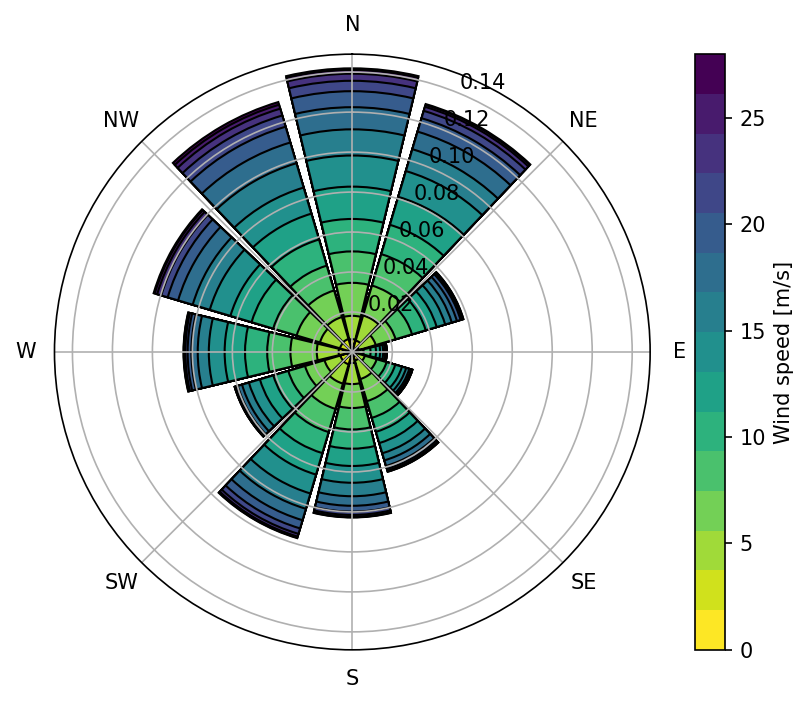
\includegraphics[width=0.65\linewidth]{wind_rose.png}
		\caption{Wind rose of the site (direction bin 30$^\circ$,
			speed bin 2\,m/s).}
		\label{fig:wind-rose}
	\end{figure}
	
	%% ─────────────────────────────────────────────────────────────────────────────
	\section{Question 2: AEP and Wind Farm Efficiency}
	%% ─────────────────────────────────────────────────────────────────────────────
	
	\subsection{Setup}
	
	For the AEP computation the wind rose was re-discretised to finer bins of
	1\,m/s (speed) and $1^\circ$ (direction), following the
	hint given in the FLORIS example files \texttt{003\_wind\_data\_objects.py} and
	\texttt{006\_get\_farm\_aep.py}.
	
	The three IEA~3.4\,MW turbines were arranged in a straight north-to-south line at
	coordinates $(x_i,\,y_i) = (0,\;i\times 5D)$ for $i = 0,1,2$, where
	$D = 130\,m$ is the rotor diameter, giving 5D spacing.  The Gauss
	Curl Hybrid (GCH) wake model with default parameters was used together with a
	wind-shear exponent of $\alpha = 0.14$ and turbulence intensity $\mathrm{TI} =
	6\,\%$.
	
	\subsection{Results}
	
	\begin{lstlisting}
		AEP (with wake):     75.603 GWh/yr
		AEP (no wake):       76.909 GWh/yr   (approx.)
		
		Capacity Factor:     71.1 %
		Wind Farm Efficiency (P / P_no_wake):  98.3 %
	\end{lstlisting}
	
	%% ─────────────────────────────────────────────────────────────────────────────
	\section{Question 3: LandBOSSE -- Balance-of-Plant and LCOE}
	%% ─────────────────────────────────────────────────────────────────────────────
	
	\subsection{LandBOSSE configuration}
	
	The \texttt{iea36\_120\_project\_data} template was selected and the following
	parameters were updated to match the assignment specification:
	
	\begin{center}
		\begin{tabular}{lrl}
			\toprule
			\textbf{Parameter} & \textbf{Value} & \textbf{Unit} \\
			\midrule
			Turbine rating         & 3.37   & MW \\
			Hub height             & 120    & m  \\
			Rotor diameter         & 130    & m  \\
			Number of turbines     & 3      & -- \\
			Turbine spacing        & 5      & $\times D$ \\
			Fuel cost              & 5.19   & USD/gal \\
			Line frequency         & 50     & Hz \\
			Array cable voltage    & 30     & kV \\
			Construction time      & 12     & months \\
			Rated thrust (computed)& 625.8  & kN \\
			\bottomrule
		\end{tabular}
	\end{center}
	
	The rated thrust was computed from the FLORIS thrust coefficient at the rated
	wind speed:
	\[
	C_{T,\text{rated}} = 0.8015, \qquad
	T = \tfrac{1}{2}\,\rho\, A\, v_{\text{rated}}^2\, C_T
	= 625.8\,kN.
	\]
	
	\newpage
	
	\subsection{Balance-of-Plant costs}
	
	\begin{lstlisting}
		
		BoP Cost (total):      $6,820,508
		
		ManagementCost       $1,519,250
		GridConnectionCost   $1,429,498
		FoundationCost       $1,095,121
		ErectionCost         $1,008,541
		SitePreparationCost    $897,342
		TransportCost          $624,000
		DevelopmentCost        $150,000
		CollectionCost          $96,755
		SubstationCost               $0
	\end{lstlisting}
	
	\subsection{Turbine capital cost and ICC}
	
	\begin{lstlisting}
		
		Turbine cost (@ $1.3 M/MW): $13,143,000
		ICC (Turbine + BoP):         $19,963,508
	\end{lstlisting}
	
	\subsection{LCOE calculation}
	
	The LCOE was evaluated with the annuity method:
	\[
	\mathrm{LCOE}
	= \frac{\mathrm{ICC}}{\mathrm{AEP}\cdot A}
	+ \frac{C_{\mathrm{O\&M}} + C_{\mathrm{land}}}{\mathrm{AEP}},
	\]
	where the annuity factor for $r = 4\,\%$ and $n = 20\,\text{yr}$ is
	\[
	A = \frac{(1+r)^n - 1}{r\,(1+r)^n} = 13.590.
	\]
	
	\begin{lstlisting}
		
		Annuity factor (4%, 20 yr):  13.590
		
		Annual O&M cost:   $1,209,642   (0.016 $/kWh * AEP)
		Annual land rental:  $202,200   (20,000 $/MW-yr * 10.11 MW)
		
		LCOE:  0.0381 $/kWh  =  38.10 $/MWh
	\end{lstlisting}
	
	%% ─────────────────────────────────────────────────────────────────────────────
	\section{Question 4: LCOE Literature Comparison and Cost Breakdown}
	%% ─────────────────────────────────────────────────────────────────────────────
	
	\subsection{Literature comparison}
	
	The computed LCOE of 38.10\,\$/MWh falls within the typical
	onshore wind range of 33--70\,\$/MWh reported by IRENA and IEA for global
	projects.  The value is towards the lower end of the European range
	(40--60\,\$/MWh) partly because the site has a high mean wind speed, yielding a
	large AEP relative to the installed capacity.
	
	\subsection{Annualised cost breakdown}
	
	\begin{lstlisting}
		
		Turbine Investment     $   967,085 /yr   33.6 %
		Balance-of-Plant       $   501,865 /yr   17.4 %
		O&M                    $ 1,209,642 /yr   42.0 %
		Land Rental            $   202,200 /yr    7.0 %
		Total                  $ 2,880,792 /yr  100.0 %
	\end{lstlisting}
	
	\begin{figure}[h!]
		\centering
		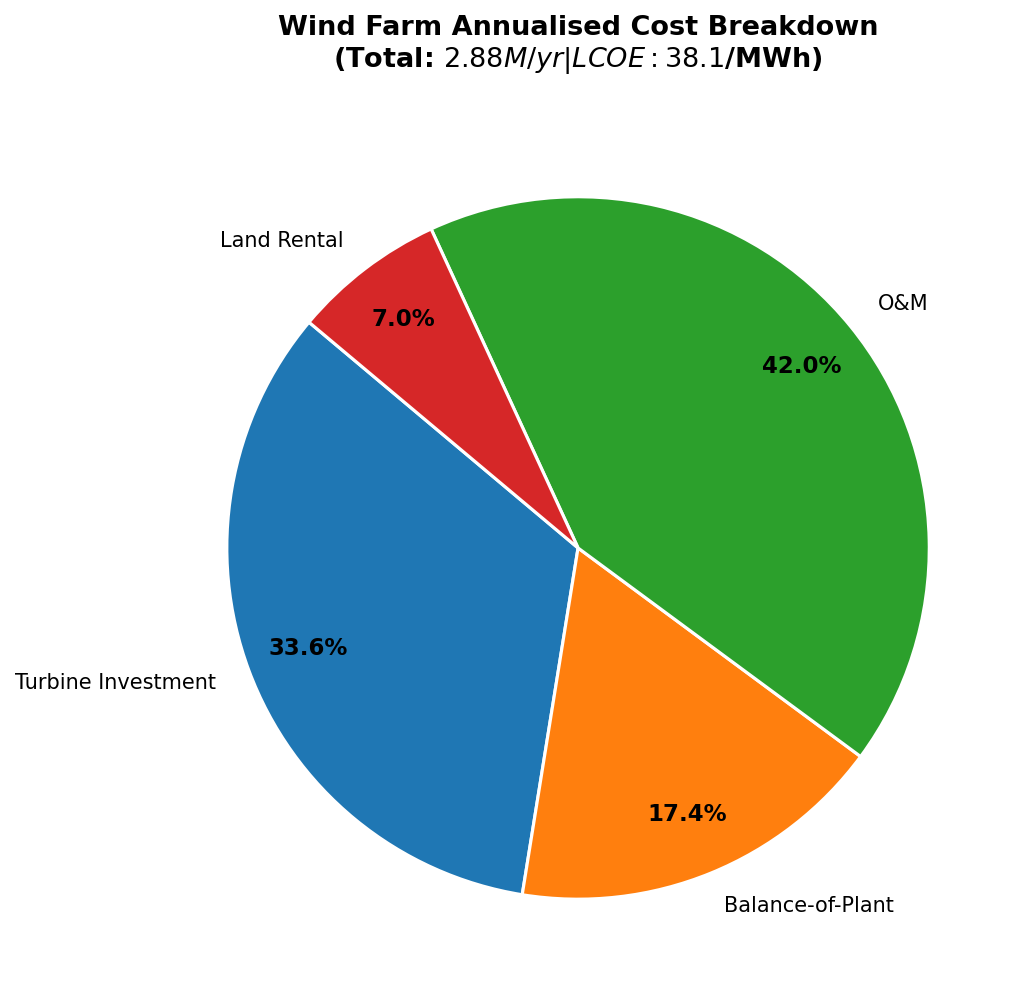
\includegraphics[width=0.58\linewidth]{cost_breakdown_pie.png}
		\caption{Annualised cost breakdown of the 3-turbine wind farm
			(total: \$2.88\,M/yr, LCOE: 38.1\,\$/MWh).}
		\label{fig:pie}
	\end{figure}
	
	O\&M dominates at 42\,\%, which is high for a three-turbine project because the
	fixed overhead (management, grid connection) is spread over a small installed
	capacity; larger farms benefit from economies of scale.
	
	%% ─────────────────────────────────────────────────────────────────────────────
	\section{Question 5: Effect of Increasing Spacing from 5D to 8D}
	%% ─────────────────────────────────────────────────────────────────────────────
	
	The turbine layout was updated to 8D spacing
	($(x_i,\,y_i) = (0,\;i\times 8D)$) and both FLORIS and LandBOSSE were
	re-run.  The substation position was adjusted accordingly
	(500\,m perpendicular to the centre of the turbine row).
	
	\begin{lstlisting}
		
		5D          8D          Relative difference w.r.t. 5D
		AEP:    75.603 GWh/yr  76.301 GWh/yr     Delta = +0.92 %
		LCOE:   38.10  $/MWh   37.94  $/MWh      Delta = -0.42 %
	\end{lstlisting}
	
	Increasing the spacing from 5D to 8D reduces wake losses (AEP rises by 0.92\,\%),
	while the BoP cost increase due to longer cable runs is small, leading to a
	marginal LCOE reduction of 0.42\,\%.  The gain is modest because the three-turbine
	layout already operates mostly out of full wake alignment, and 5D provides
	sufficient recovery for the dominant wind directions at this site.
	
	%% ─────────────────────────────────────────────────────────────────────────────
	\section{Question 6: Effect of a Reduced Discount Rate}
	%% ─────────────────────────────────────────────────────────────────────────────
	
	If the discount rate decreases by 10\,\% (from $r = 4\,\%$ to
	$r = 3.6\,\%$), the annuity factor increases, meaning future revenues are
	discounted less steeply and the amortised capital cost is spread more
	favourably.
	
	\begin{lstlisting}
		
		LCOE @ 4.0 %:   38.104 $/MWh
		LCOE @ 3.6 %:   37.422 $/MWh
		Delta:           -1.790 %
	\end{lstlisting}
	
	A 10\,\% relative reduction in the discount rate translates into a 1.79\,\%
	reduction in LCOE.  Capital-intensive projects are more sensitive to the
	financing rate than fuel-cost-driven plants; however, for a modest three-turbine
	farm dominated by O\&M costs the sensitivity is still limited.
	
	%% ─────────────────────────────────────────────────────────────────────────────
	\section{Question 7: AEP Improvement Strategy}
	%% ─────────────────────────────────────────────────────────────────────────────
	
	\subsection{Proposed method: staggered layout}
	
	The turbines were repositioned from a pure north-to-south line to a staggered
	arrangement in the cross-wind direction:
	\[
	(x_i,\,y_i) = \bigl(\;0,\;+5D,\;-5D\bigr) \times \bigl(0,\;5D,\;10D\bigr).
	\]
	By offsetting turbines laterally, the downstream rotors no longer sit in the
	centre of the upstream wake, which increases their inflow velocity for the
	dominant wind directions.
	
	\begin{lstlisting}
		
		Baseline AEP (in-line):      75.603 GWh
		Staggered AEP:               76.304 GWh
		AEP improvement:              0.928 %
	\end{lstlisting}
	
	\subsection{Discussion}
	
	The 0.93\,\% gain is meaningful for a small farm.  At larger scale, staggered or
	fully optimised layouts routinely deliver 2--5\,\% AEP improvement over a regular
	grid.  Other strategies that can be applied to an already-installed farm (without
	repositioning turbines) include:
	\begin{itemize}[leftmargin=1.5em]
		\item \textbf{Wake steering (yaw control)}: intentionally misaligning upstream
		turbines to deflect their wakes away from downstream rotors.
	\end{itemize}
	
	%% ─────────────────────────────────────────────────────────────────────────────
	\section{Question 8: IRR and Profitability Index}
	%% ─────────────────────────────────────────────────────────────────────────────
	
	\subsection{Revenue and cash-flow}
	
	The average electricity spot price over the project lifetime is
	41.8\,\$/MWh.
	
	\begin{lstlisting}
		
		Annual Revenue:       $3,160,190   (41.8 $/MWh * 75,603 MWh)
		Annual O&M Cost:      $1,209,642
		Annual Land Rental:   $  202,200
		Annual Net Cash Flow: $1,748,348
		Initial Investment:   $19,963,508
	\end{lstlisting}
	
	\subsection{NPV and IRR}
	
	The Net Present Value for a constant annual cash flow $C$ over $n$ years at
	discount rate $r$ is
	\[
	\mathrm{NPV}(r) = C\,\frac{(1+r)^n - 1}{r(1+r)^n} - I_0.
	\]
	The Internal Rate of Return is the root of $\mathrm{NPV}(r)=0$, found numerically by Brent's method. The graph for the same is seen in Figure 3.
	
	\begin{lstlisting}
		
		IRR:  6.055 %
	\end{lstlisting}
	
	\begin{figure}[h!]
		\centering
		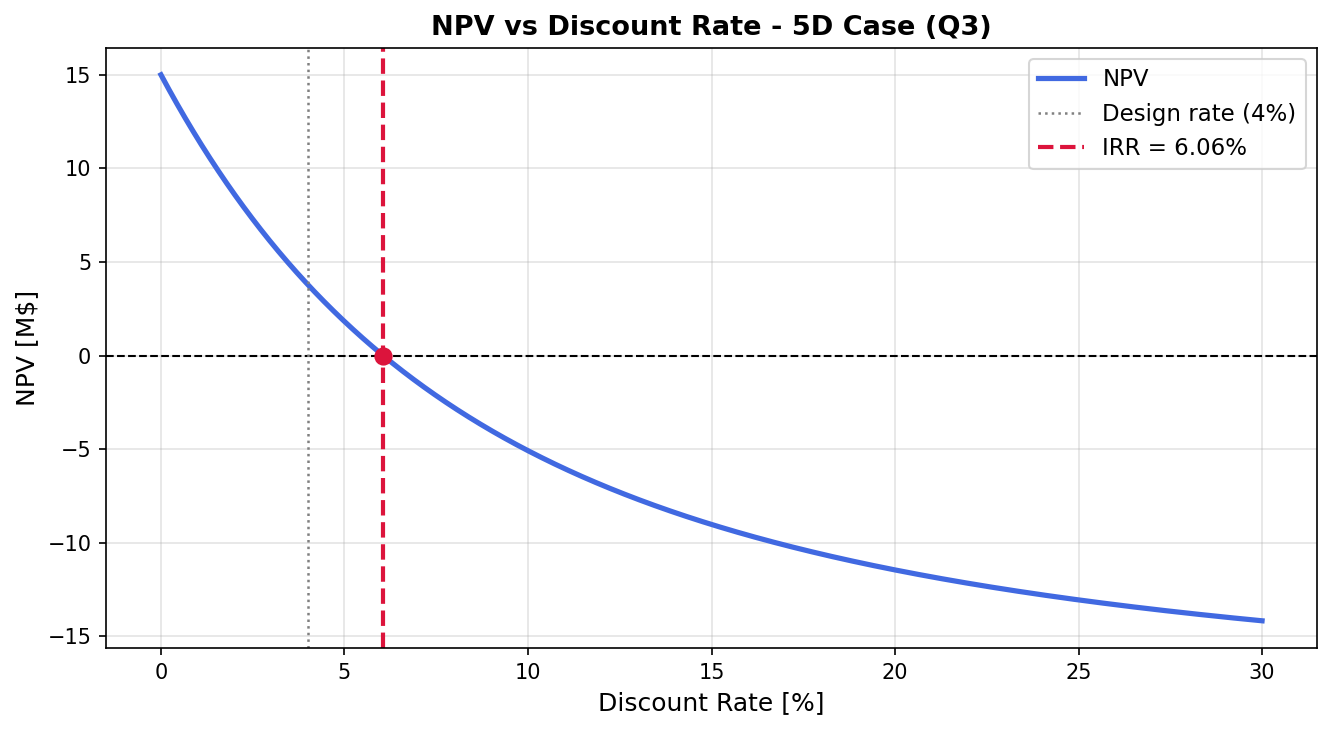
\includegraphics[width=0.82\linewidth]{q8_npv_vs_discount_rate_irr.png}
		\caption{NPV vs.\ discount rate for the 5D case (Q3).
			The IRR of 6.06\,\% is marked where NPV crosses zero.}
		\label{fig:npv-irr}
	\end{figure}
	
	\subsection{Profitability Index}
	
	The Profitability Index is
	\[
	\mathrm{PI} = \frac{\mathrm{PV(cash\;flows)}}{I_0}
	= 1 + \frac{\mathrm{NPV}}{I_0}.
	\]
	
	\begin{lstlisting}
		
		PV of cash flows (@4%):   $23,760,617
		Initial Investment:       $19,963,508
		NPV @ 4%:                  $3,797,109
		PI:                            1.1902
	\end{lstlisting}
	
	\subsection{Economic assessment}
	
	The project is \textbf{economically attractive}: PI $= 1.19 > 1$ and
	IRR $= 6.06\,\% > r = 4\,\%$.  The IRR exceeds the discount rate, confirming
	that the project creates value for investors.  If, however, the electricity
	price were lower (e.g.\ at market prices closer to the LCOE), the project would
	break even at best.  Ways to improve viability in a lower-price environment
	include subsidies or feed-in tariffs, a higher electricity selling price via a
	Power Purchase Agreement, or reducing CAPEX through economies of scale.
	
	%% ─────────────────────────────────────────────────────────────────────────────
	\section{Question 9: Minimum Turbines for PI $>$ 1}
	%% ─────────────────────────────────────────────────────────────────────────────
	
	\subsection{Methodology}
	
	The turbine count was varied from 1 to 10 in a straight north-to-south line with
	5D spacing.  For each count, FLORIS computed the AEP and LandBOSSE recomputed the
	BoP costs; then the PI was evaluated at $r = 4\,\%$ and $n = 20\,\text{yr}$ using
	the same electricity price of 41.8\,\$/MWh.
	
	\subsection{Results}
	
	\begin{center}
		\begin{tabular}{crrrrr}
			\toprule
			$N$ & ICC [\$M] & PV CFs [\$M] & NPV [\$M] & PI \\
			\midrule
			1  & 11.20 &  6.24 & $-$4.96 & 0.558 \\
			2  & 15.58 & 13.75 & $-$1.83 & 0.883 \\
			\textbf{3} & \textbf{19.96} & \textbf{20.86} & \textbf{0.89} & \textbf{1.045} \\
			4  & 24.34 & 27.79 & 3.44 & 1.141 \\
			5  & 28.73 & 34.62 & 5.90 & 1.205 \\
			6  & 33.11 & 41.39 & 8.28 & 1.250 \\
			7  & 37.49 & 48.13 &10.64 & 1.284 \\
			8  & 41.87 & 54.83 &12.96 & 1.310 \\
			9  & 46.25 & 61.51 &15.26 & 1.330 \\
			10 & 50.63 & 68.18 &17.55 & 1.347 \\
			\bottomrule
		\end{tabular}
	\end{center}
	
	\vspace{0.4em}
	The minimum number of turbines to achieve PI\,$>$\,1 is \textbf{3 turbines}.
	
	\begin{figure}[h!]
		\centering
		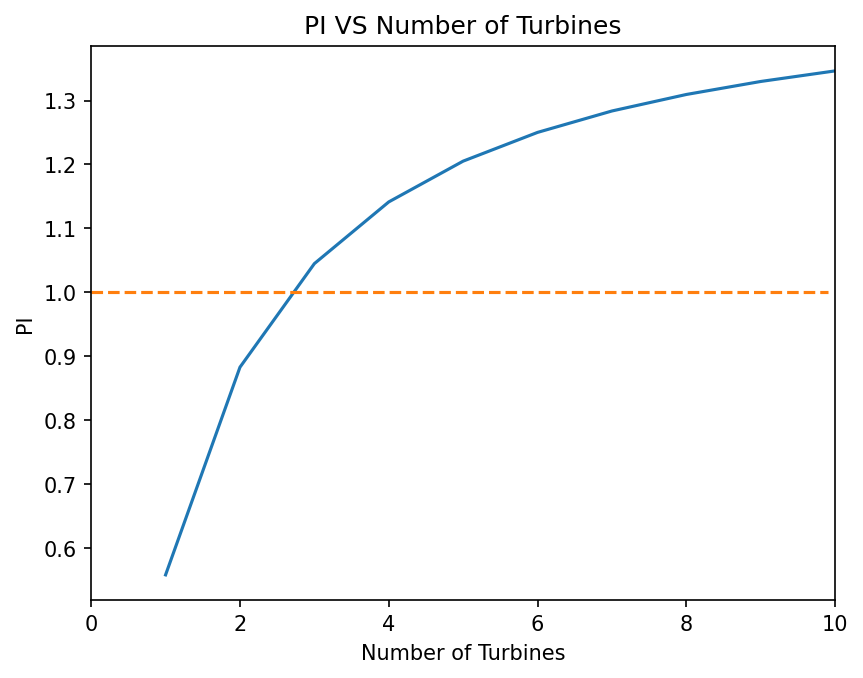
\includegraphics[width=0.78\linewidth]{q9_pi_vs_turbines.png}
		\caption{Profitability Index vs.\ number of turbines.
			The dashed line marks PI $= 1$.}
		\label{fig:pi-turbines}
	\end{figure}
	
	\begin{figure}[h!]
		\centering
		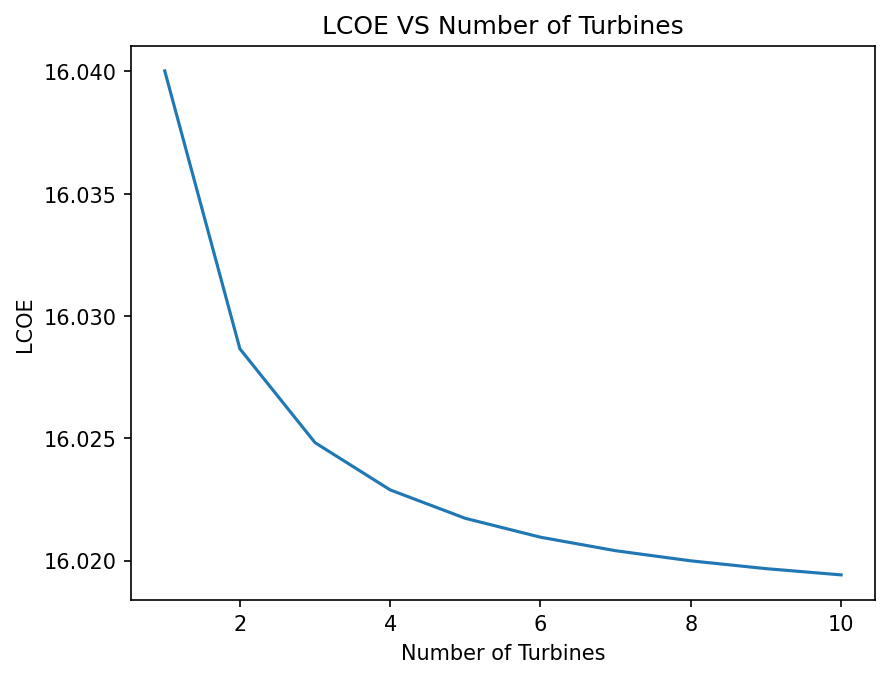
\includegraphics[width=0.78\linewidth]{q9_lcoe_vs_turbines.png}
		\caption{LCOE vs.\ number of turbines.}
		\label{fig:lcoe-turbines}
	\end{figure}
	
	\subsection{Discussion}
	
	Both PI and LCOE improve monotonically as the number of turbines grows,
	reflecting the economies of scale in the BoP costs. The
	marginal benefit diminishes as $N$ increases, so there is a practical optimum
	that also takes land constraints, grid capacity, and permitting into account.
	With only 1 or 2 turbines the project destroys value because the fixed BoP costs
	dominate the relatively small revenue.
	
\end{document}